% -*- coding: utf-8 -*-

\documentclass[a4paper,dvipdfmx]{jsarticle}
\usepackage{ascmac,alltt,txfonts,url}

\usepackage[dvipdfmx]{graphicx}
\usepackage{here}
\usepackage{fancyvrb}

\renewcommand{\ttdefault}{cmtt}
\renewcommand{\figurename}{図} 
\renewcommand{\tablename}{表} 
\DeclareMathAlphabet{\mathtt}{OT1}{cmtt}{m}{n}
\SetMathAlphabet{\mathtt}{bold}{OT1}{cmtt}{m}{n}
\setlength{\oddsidemargin}{0cm}
\setlength{\evensidemargin}{0cm}

\makeatletter

\newdimen\@mojihaba
\settowidth{\@mojihaba}{あ}

\def\tokushu#1{%
\def\tokushutitle{#1}%
\gdef\articleHeader{\hbox to\textwidth{\rule{3\@mojihaba}{1mm}%
\hbox{\small\bf\hskip1mm \tokushutitle}\leaderfill}}
}

\newdimen \JQ	\JQ .259817mm	%%%	\JQ/\Q = 10pt/9.62216pt
\newdimen \Q	\Q  .25mm	%%%	Quarter of 1mm

\def\JarticleHeader{\rule{\textwidth}{1mm}}%
\def\JarticleTitle{{\huge\bf\@title}}
\def\JarticleAuthor{\large\begin{tabular}[t]{@{}l}\@author\end{tabular}}
\newbox\@temptitlebox

\def\verse{\let\\=\@centercr 
 \list{}{\itemsep\z@ \itemindent -1.5em\listparindent \itemindent 
 \rightmargin\leftmargin\advance\leftmargin 1.5em}\item[]}
\let\endverse\endlist
\def\quotation{\list{}{\listparindent 1.5em
 \itemindent\listparindent
 \rightmargin\leftmargin \parsep 0pt plus 1pt}\item[]}
\let\endquotation=\endlist
\def\quote{\list{}{\rightmargin\leftmargin}\item[]}
\let\endquote=\endlist
\def\abstquotation{\list{}{\listparindent 1.5em
 \itemindent\listparindent
 \leftmargin 5mm
 \rightmargin\leftmargin \parsep 0pt plus 1pt}\item[]}
\let\endabstquotation=\endlist
\def\quote{\list{}{\rightmargin\leftmargin}\item[]}
\let\endquote=\endlist

\global\def\@maketitle{\newpage \null
\hbox{\vbox to193.5\Q{\baselineskip=10mm % 193.5\Q = 9*\baselineskip
\begin{flushleft}
\JarticleHeader
% following extra vskip together with baselineskip(10mm) will produce
% appropriate 10mm/6mm gap between the rule and title
% This assumes that title is typeset with 28Q(7mm) font, and baseline
% is set 1mm above the bottom of the font.
\setbox\@temptitlebox\hbox{JarticleTitle}\ifdim\wd\@temptitlebox>\textwidth\vskip2mm\else\vskip6mm\fi
\leftskip=5mm
\JarticleTitle
\vskip6mm % to leave 10mm gap between title and author
\JarticleAuthor
\end{flushleft}\vfil}}
%\JEabstInsert
  \begin{small}
    \begin{abstquotation}
      \Jabstcontent
    \end{abstquotation}
  \end{small}
}

\long\def\Jabstract#1{\global\long\def\Jabstcontent{\noindent\ignorespaces #1}}
\def\Jabstcontent{\relax}

\makeatother

\usepackage{fancyhdr}
\pagestyle{fancy}
\lhead{アプリケーション実験}
\rhead{}
\rhead{\thepage{}}
\cfoot{}
\renewcommand{\headrulewidth}{0.5pt}
\pagestyle{fancy}

\Jabstract{%
\\
HDLのいろいろな記述方法を使って,少し複雑なモジュールの設計に取り組んでみましょう.
}

\begin{document}

\title{アプリケーション実験}
\author{}
\date{2019年 1月14日~~第3.0版}
\maketitle

\section{はじめに}
これまでに学んできた内容を利用して,少し応用的な実験に取り組んでみましょう.

\section{ストップウォッチを作ってみよう}
ここでは,
\begin{itemize}
 \item アクションボタンを押すとミリ秒毎のカウントアップを開始する
 \item カウント中に,アクションボタンを押すとカウントを一時停止する
 \item 一時停止中に,アクションボタンを押すとカウントを再開する
 \item リセットボタンを押すとカウントを0にクリアする
\end{itemize}
という機能をもったストップウォッチを作ってみましょう.

残念ながら,ZYBO Z7-20には,7セグメントLEDのような数字を表示する分かりやすい表示器はありませんので,4つのLEDと2つの3色LEDを使って数を表現するとよいでしょう.

次のリストはストップウォッチを実装するためのトップモジュールの例です.3色LEDの明るさを適当に調節するために,PWMモジュールを使って出力を変調しています.PWMモジュールによって,たとえば\verb|'1'|を出力する場合でも,適当なタイミングで'1'と'0'がまぜられることで明るさを抑えることができます.

\begin{figure}[H]
\begin{quote}
\begin{Verbatim}[frame=single, numbers=left, baselinestretch=0.8]
library ieee;
use ieee.std_logic_1164.all;
use ieee.numeric_std.all;

entity stopwatch_z7_20 is
  port (
    CLK : in  std_logic;

    led6_r : out std_logic;
    led6_g : out std_logic;
    led6_b : out std_logic;
    
    led5_r : out std_logic;
    led5_g : out std_logic;
    led5_b : out std_logic;

    LD : out std_logic_vector(3 downto 0);
    
    btn : in std_logic_vector(1 downto 0)
    );
  
end entity stopwatch_z7_20;

architecture RTL of stopwatch_z7_20 is

  attribute ASYNC_REG : string;
  attribute mark_debug : string;

  component stopwatch
    generic (
      FREQ_MHz : integer := 125
      );
    port (
      clk      : in  std_logic;
      reset    : in  std_logic;
      action   : in  std_logic;
      msec_out : out std_logic_vector(9 downto 0);
      sec_out  : out std_logic_vector(5 downto 0);
      min_out  : out std_logic_vector(5 downto 0);
      hour_out : out std_logic_vector(4 downto 0)
      );
  end component stopwatch;

  component pwm
    port (
\end{Verbatim}
\end{quote}
\end{figure}
次のページに続く
\begin{figure}[H]
\begin{quote}
\begin{Verbatim}[frame=single, numbers=left, baselinestretch=0.8]
      clk : in  std_logic;
      a   : in  std_logic_vector(3 downto 0);
      d   : in  std_logic;
      q   : out std_logic
      );
  end component pwm;

  signal btn_d0 : std_logic_vector(1 downto 0);
  signal btn_d1 : std_logic_vector(1 downto 0);
  
  attribute ASYNC_REG of btn_d0, btn_d1 : signal is "TRUE";

  signal msec_out : std_logic_vector(9 downto 0);
  signal sec_out  : std_logic_vector(5 downto 0);
  signal min_out  : std_logic_vector(5 downto 0);
  signal hour_out : std_logic_vector(4 downto 0);

  attribute mark_debug of msec_out : signal is "true";
  attribute mark_debug of sec_out  : signal is "true";
  attribute mark_debug of min_out  : signal is "true";
  attribute mark_debug of hour_out : signal is "true";

begin

  process(CLK)
  begin
    if rising_edge(CLK) then
      btn_d0 <= btn;
      btn_d1 <= btn_d0;
    end if;
  end process;

  U: stopwatch
    generic map(
      FREQ_MHz => 125
      )
    port map(
      clk      => CLK,
      reset    => btn_d1(0),
      action   => btn_d1(1),
      msec_out => msec_out,
      sec_out  => sec_out,
      min_out  => min_out,
      hour_out => hour_out
      );
\end{Verbatim}
\end{quote}
\end{figure}
次のページに続く
\begin{figure}[H]
\begin{quote}
\begin{Verbatim}[frame=single, numbers=left, baselinestretch=0.8]

  LD <= sec_out(3 downto 0);
  
  PWM0 : pwm
    port map(clk => clk, a => "1100", d => msec_out(0), q => led5_r);
  PWM1 : pwm
    port map(clk => clk, a => "1100", d => msec_out(1), q => led5_g);
  PWM2 : pwm
    port map(clk => clk, a => "1100", d => msec_out(2), q => led5_b);
  PWM3 : pwm
    port map(clk => clk, a => "1100", d => msec_out(3), q => led6_r);
  PWM4 : pwm
    port map(clk => clk, a => "1100", d => msec_out(4), q => led6_g);
  PWM5 : pwm
    port map(clk => clk, a => "1100", d => msec_out(5), q => led6_b);

end RTL;
\end{Verbatim}
\end{quote}
\end{figure}

\verb|stopwatch|モジュールを実装して,完成させてみましょう.

\section{シリアル通信に挑戦してみよう}

最近のパソコンの外部機器のI/OのほとんどはUSBです.ノート・パソコンは勿論,省スペースのデスクトップ・パソコンにさえ,RS-232-Cのシリアル通信のポートが搭載されなくなってきました.それでも,送信と受信の2本で通信可能なRS-232-Cは,パソコンとFPGAの間やFPGAとFPGAの間でデータを手軽にやりとりする手段として基本的かつ必要不可欠な存在です.

シリアル・ポートのないノート・パソコンでも,市販のUSB-シリアル変換ケーブルやBluetooth-シリアル変換モジュールを使って簡単に接続できます.

\subsection{シリアル通信のしくみ}
シリアル通信では,受信と送信で独立したポートを持ちます.機器を直結する場合には,お互いの送受信ポートをクロスして結線します(図\ref{fig:serial_comm}).

 \begin{figure}[H]
  \begin{center}
   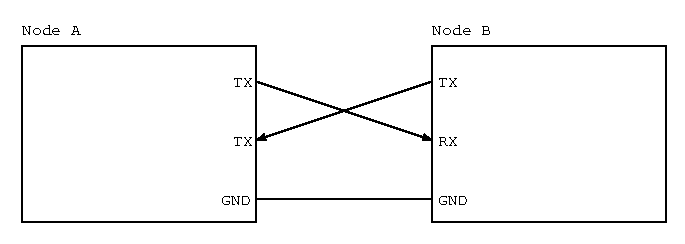
\includegraphics[width=.6\textwidth]{chapter06_figures/serial_comm.eps}
  \end{center}  
  \caption{シリアル通信の結線\label{fig:serial_comm}}
 \end{figure}

RS-232-Cでは,図\ref{serial_comm_format}のように,8ビットのデータにスタート・ビット('0')とストップ・ビット('1')を付加してデータを通信します.接続した機器同士であらかじめ決めた速度(たとえば19200bpsなど)で信号を送受信することで,共通したクロックを持つことなくデータの送受信ができます.

 \begin{figure}[H]
  \begin{center}
   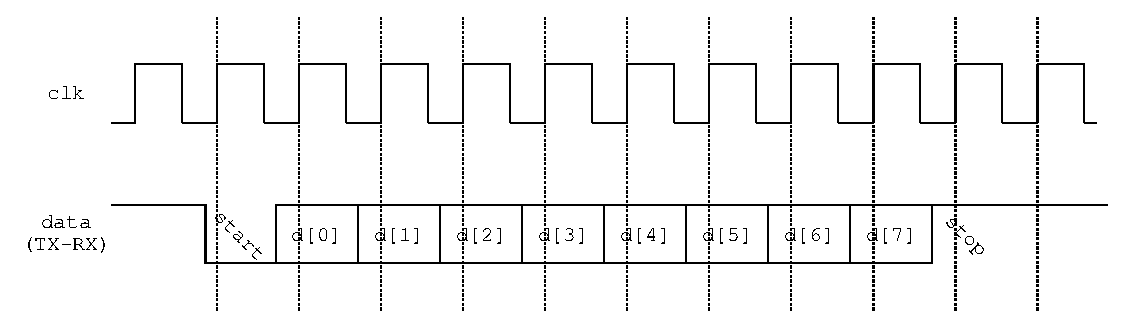
\includegraphics[width=.6\textwidth]{chapter06_figures/serial_comm_format.eps}
  \end{center}  
  \caption{シリアル通信の結線\label{fig:serial_comm_format}}
 \end{figure}

\subsection{送信モジュール}
決められた速度で信号をパタパタと変化させるだけです.ただし,一般に,シリアル通信の速度は回路の動作クロックに対して,とても遅いので,データを送信している途中に送るべき信号を更新してしまわないようにブロックする仕組みが必要です.VHDLによる実装例を示します.

\begin{figure}[H]
\begin{quote}
\begin{Verbatim}[frame=single, numbers=left, baselinestretch=0.8]
library ieee;
use ieee.std_logic_1164.all;
use ieee.numeric_std.all;

entity uart_tx is
  -- 定数宣言
  generic (
    sys_clk : integer := 14000000;             --クロック周波数
    rate    : integer := 9600                  --転送レート,単位はbps(ビット毎秒)
    );
  -- 入出力ポート宣言
  port (
    clk   : in  std_logic;                     -- クロック
    reset : in  std_logic;                     -- リセット
    wr    : in  std_logic;                     -- 送信要求
    din   : in  std_logic_vector(7 downto 0);  --送信データ
    dout  : out std_logic;                     --シリアル出力
    ready : out std_logic                      --送信要求を受け付けられるか
    );
end uart_tx;

architecture rtl of uart_tx is
  -- クロック分周モジュールの呼び出しの準備
  component clk_div is
    port (clk     : in  std_logic;
          rst     : in  std_logic;
          div     : in  std_logic_vector(15 downto 0);
          clk_out : out std_logic);
  end component;
  -- 内部変数定義
  signal in_din : std_logic_vector(7 downto 0);  -- 送信データ一時保存用レジスタ
  signal buf    : std_logic_vector(7 downto 0);  -- 一時的にしようするバッファ
  signal load   : std_logic := '0';              -- 送信データを読み込んだかどうか
  signal cbit   : unsigned(2 downto 0) := (others => '0');  -- 送信するビット番号

  signal run : std_logic := '0';               -- 送信状態にあるかどうか

  signal tx_en   : std_logic; -- 送信用クロック
  signal tx_en_d : std_logic := '0'; -- 送信用クロックの立ち上がり検出用
  
  signal tx_div : std_logic_vector(15 downto 0); -- クロック分周の倍率

  signal status : unsigned(1 downto 0); -- 状態遷移用レジスタ

begin
\end{Verbatim}
\end{quote}
\end{figure}
次のページに続く

\begin{figure}[H]
\begin{quote}
\begin{Verbatim}[frame=single, numbers=left, baselinestretch=0.8]
  -- クロック分周モジュールの呼び出し
  -- clk_divの入出力ポートにこのモジュールの内部変数を接続
  tx_div <= std_logic_vector(to_unsigned((sys_clk / rate) - 1, 16));
  U0 : clk_div port map (clk=>clk, rst=>reset, div=>tx_div, clk_out=>tx_en);

  -- readyへの代入, 常時値を更新している
  ready  <= '1' when (wr = '0' and run = '0' and load = '0') else '0';

  process(clk) --変化を監視する信号を記述する, この場合クロック
  begin
    if rising_edge(clk) then  --クロックの立ち上がり時の動作
      if reset = '1' then                 --リセット時の動作, 初期値の設定
        load <= '0';
      else
        if(wr = '1' and run = '0') then    --送信要求があり,かつ送信中でない場合
          load   <= '1';                   --データを取り込んだフラグを立てる
          in_din <= din;                   --一時保存用レジスタに値を格納
        end if;
        if(load = '1' and run = '1') then  --送信中で,かつデータを取り込んだ
                                           --ことを示すフラグが立っている場合
          load <= '0';                     --データを取り込んだフラグを下げる
        end if;
      end if;
    end if;
  end process;

  process(clk)                            --変化を監視する信号(クロック)
  begin
    if rising_edge(clk) then
      if reset = '1' then                 --リセット時の動作, 初期値の設定
        dout    <= '1';
        cbit    <= (others => '0');
        status  <= (others => '0');
        run     <= '0';
        tx_en_d <= '0';
      else
        tx_en_d <= tx_en;
        if tx_en = '1' and tx_en_d = '0' then -- tx_enの立ち上がりで動作
          case to_integer(status) is        --statusの値に応じて動作が異なる
            when 0          =>              --初期状態
              cbit <= (others => '0');        --カウンタをクリア
              if load = '1' then              -- データを取り込んでいる場合
                dout   <= '0';                -- スタートビット0を出力
                status <= status + 1;         -- 次の状態へ
                buf    <= in_din;             -- 送信データを一時バッファに退避
\end{Verbatim}
\end{quote}
\end{figure}
次のページに続く
\begin{figure}[H]
\begin{quote}
\begin{Verbatim}[frame=single, numbers=left, baselinestretch=0.8]
                run    <= '1';                -- 送信中の状態へ遷移
              else                            --なにもしない状態へ遷移
                dout <= '1';
                run  <= '0';                  --送信要求受付可能状態へ
              end if;
            when 1 =>                         --データをLSBから順番に送信
              cbit <= cbit + 1;               -- カウンタをインクリメント
              dout <= buf(to_integer(cbit));  --一時バッファのcbit目を取出して出力
              if(to_integer(cbit) = 7) then   -- データの8ビット目を送信したら,
                                              -- ストップビットを送る状態へ遷移
                status <= status + 1;
              end if;
            when 2 =>                         -- ストップビットを送信
              dout   <= '1';                  --ストップビット1
              status <= (others => '0');      --初期状態へ
            when others =>                    --その他の状態の場合
              status <= (others => '0');      -- 初期状態へ遷移
          end case;
        end if;
      end if;
    end if;
  end process;

end rtl;
\end{Verbatim}
\end{quote}
\end{figure}

内部で利用している\verb|clk_div|の実装は次の通りです.
\begin{figure}[H]
\begin{quote}
\begin{Verbatim}[frame=single, numbers=left, baselinestretch=0.8]
library ieee;
use ieee.std_logic_1164.ALL;
use ieee.numeric_std.all;

entity clk_div is
  port(
    clk     : in  std_logic;
    rst     : in  std_logic;
    div     : in  std_logic_vector(15 downto 0);
    clk_out : out std_logic
    );
end clk_div;

architecture RTL of clk_div is

  signal counter : unsigned(15 downto 0) := (others => '0');

begin

  process(clk)
  begin
    if(clk'event and clk = '1') then
      if(rst = '1') then
        counter <= (others => '0');
      elsif (counter = unsigned(div)) then
        counter <= (others => '0');
        clk_out <= '1';
      else
        counter <= counter + 1;
        clk_out  <= '0';
      end if;
    end if; 
  end process;

end RTL;
\end{Verbatim}
\end{quote}
\end{figure}

\verb|clk_div|モジュールで生成した,シリアル送信用の信号にあわせて,送信すべきデータを1bitずつ出力します.
また,出力中はready信号を'0'にすることで,送信モジュールが動作中であることを上位のモジュールに伝えられるようになっています.

このモジュールの動作をシミュレーションで確認してみましょう.

\subsection{受信モジュール}
受信モジュールは送信モジュールに比べて少し複雑になります.送信側は自分のタイミングで信号を送ればいいのに対し,受信側ではスタート・ビットを頼りにデータの開始を検出し,以降の信号を正しい間隔でビットに分割しなければならないからです.また,データにはノイズが乗っている可能性もあるので,データを正しく取得する仕組みも必要です.
VHDLとVerilog HDLによる実装の例が次のリストです.この例では,通信速度の16倍のクロックでデータをサンプリング(一定間隔で読み込む)することで,データを受信しています.

\begin{figure}[H]
\begin{quote}
\begin{Verbatim}[frame=single, numbers=left, baselinestretch=0.8]
library ieee;
use ieee.std_logic_1164.all;
use ieee.numeric_std.all;

entity uart_rx is
  -- 定数宣言
  generic(
    sys_clk : integer := 14000000;            --クロック周波数
    rate    : integer := 9600                 --転送レート,単位はbps(ビット毎秒)
    );
  -- 入出力ポート宣言
  port(
    clk   : in  std_logic;                    -- クロック
    reset : in  std_logic;                    -- リセット
    din   : in  std_logic;                    -- シリアル入力
    rd    : out std_logic;                    -- 受信完了を示す
    dout  : out std_logic_vector(7 downto 0)  -- 受信データ
    );
end uart_rx;

architecture rtl of uart_rx is

  --クロック分周モジュールのインスタンス生成の準備
  component clk_div is
    port(
      clk     : in  std_logic;
      rst     : in  std_logic;
      div     : in  std_logic_vector(15 downto 0);
      clk_out : out std_logic
      );
  end component;
  --内部変数宣言
  signal buf       : std_logic_vector(7 downto 0);   --受信データ系列の一時保存用
  signal receiving : std_logic;         --受信しているかどうか
  signal cbit      : integer range 0 to 150; -- データの取り込みタイミング用カウンタ
  signal rx_en     : std_logic;         --受信用クロック
  signal rx_en_d   : std_logic := '0';  --受信用クロック立ち上がり判定用レジスタ
  signal rx_div    : std_logic_vector(15 downto 0);  --クロック分周の倍率

begin
  --クロック分周モジュールのインスタンス生成
  --受信側は送信側の16倍の速度で値を取り込み処理を行う
  rx_div <= std_logic_vector(to_unsigned(((sys_clk / rate) / 16) - 1, 16));
  U0 : clk_div port map (clk=>clk, rst=>reset, div=>rx_div, clk_out=>rx_en);

\end{Verbatim}
\end{quote}
\end{figure}
次のページに続く
\begin{figure}[H]
\begin{quote}
\begin{Verbatim}[frame=single, numbers=left, baselinestretch=0.8]
  process(clk)                          --変化を監視する信号を記述,この場合クロック
  begin
    if rising_edge(clk) then
      if reset = '1' then               --リセット時の動作, 初期値の設定
        receiving <= '0';
        cbit      <= 0;
        buf       <= (others => '0');
        dout      <= (others => '0');
        rd        <= '0';
        rx_en_d   <= '0';
      else
        rx_en_d <= rx_en;
        if rx_en = '1' and rx_en_d = '0' then   --受信用クロック立ち上がり時の動作
          if receiving = '0' then       --受信中でない場合
            if din = '0' then           --スタートビット0を受信したら
              rd <= '0';                --受信完了のフラグをさげる
              receiving <= '1';
            end if;
          else                          --受信中の場合
            case cbit is                --カウンタに合わせてデータをラッチ
              when 6 =>                 -- スタートビットのチェック
                if din = '1' then       -- スタートビットが中途半端.入力をキャンセル
                  receiving <= '0';
                  cbit      <= 0;
                else
                  cbit <= cbit + 1;
                end if;
              when 22 | 38 | 54 | 70 | 86 | 102 | 118 | 134 =>  --data
                cbit <= cbit + 1;
                buf  <= din & buf(7 downto 1);  -- 新しい入力と受信済みデータを連結
              when 150 =>               --stop
                rd        <= '1';
                dout      <= buf;
                receiving <= '0';       -- 受信完了
                cbit      <= 0;
              when others =>
                cbit <= cbit + 1;
            end case;
          end if;
        end if;
      end if;
    end if;
  end process;

end RTL;
\end{Verbatim}
\end{quote}
\end{figure}
通信速度の16倍でデータをサンプリングしているので,スタート・ビットは16サイクル分が取得できるはずです.スタートビットのはじまりと思われる'0'というデータを確認してから6サイクル目のデータをもう一度取得し,そのデータがやっぱり'0'であれば,データ送信が開始されたと解釈します(ソース・コード中の状態1).データが送信されていることを確認した後は,16サイクル毎にデータを取得します(ソース・コード中の状態2).8bit分データを取得したら完了です.

送信モジュールと同じように,テストベンチを書いてシミュレーションで動作を確認してみましょう.

\subsection{実機で動作確認}
シリアル通信を実機で動作確認してみましょう.入出力にPMODコネクタJEの1ピンと7ピンを割当て,物理的に両者をジャンパピンで接続すれば,通信ができるはずです.動作をILAを使って確認してみましょう.{\bf 注意: PMODコネクタの6ピンと12ピンは3.3V,5ピンと11ピンはGNDです.間違って6ピンと5ピンなどのように3.3VとGNDを直結しないようにしましょう.}

 \begin{figure}[H]
  \begin{center}
   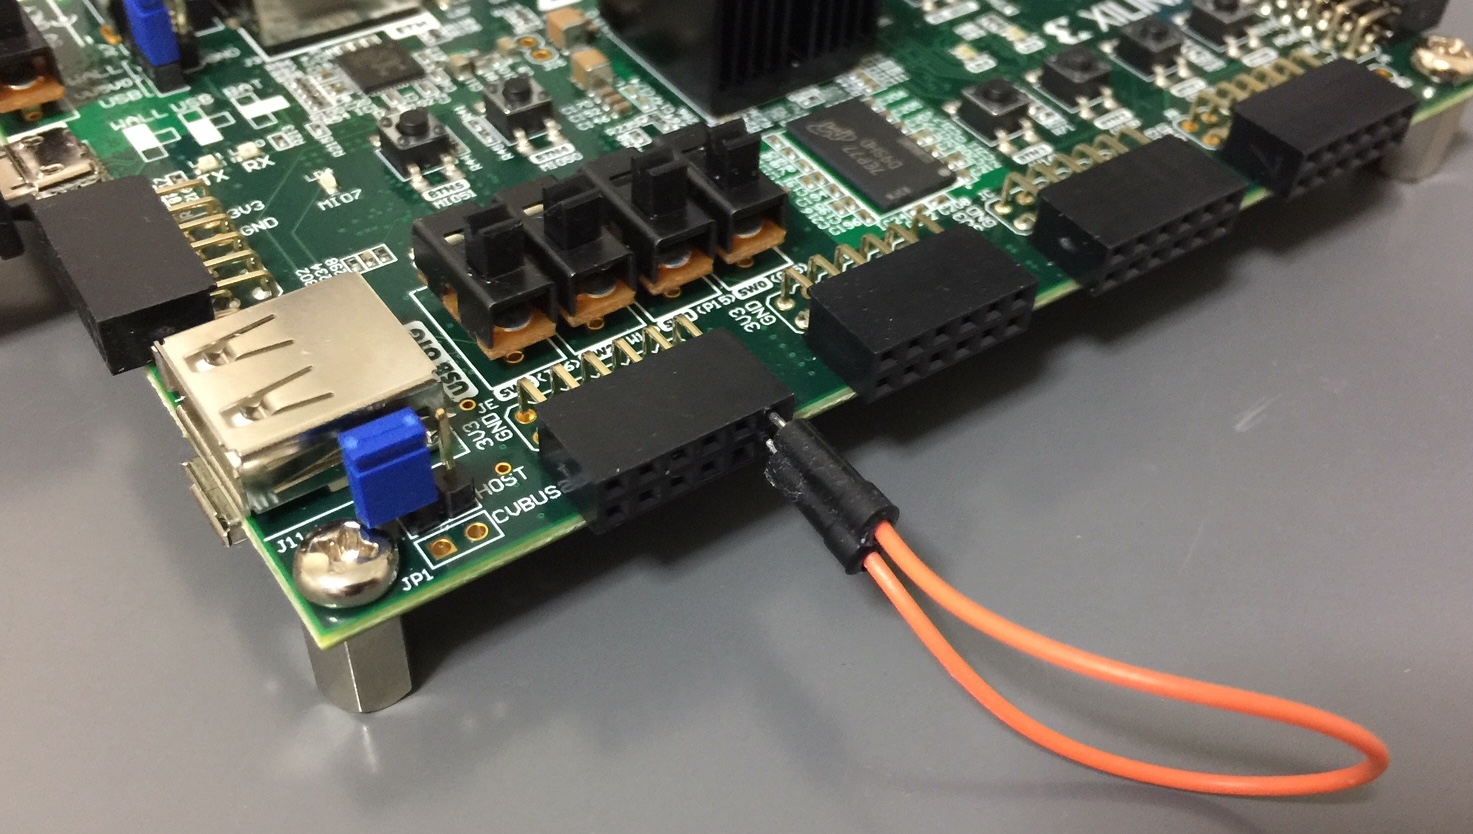
\includegraphics[width=.6\textwidth]{chapter06_figures/IMG_0007.JPG}
  \end{center}
  \label{fig:serial_comm_test}
  \caption{PMODコネクタのJEの1ピンと7ピンをジャンパケーブルで接続した様子}
 \end{figure}

\section{音声信号を観測してみよう}\label{sec:ssm2603_input}

ZYBO Z7-20には音声入出力用のジャックが備わっています.これを利用すると外部からの音声信号を取り込みFPGAで処理することができます.信号は,SSM2603というICでA/D変換されます.SSM2603とFPGAはI2Sで音声データをやりとりすることができます.

SSM2603とやりとりするI2S信号は図\ref{fig:ssm2603_protocol}の通りです.
 \begin{figure}[H]
  \begin{center}
   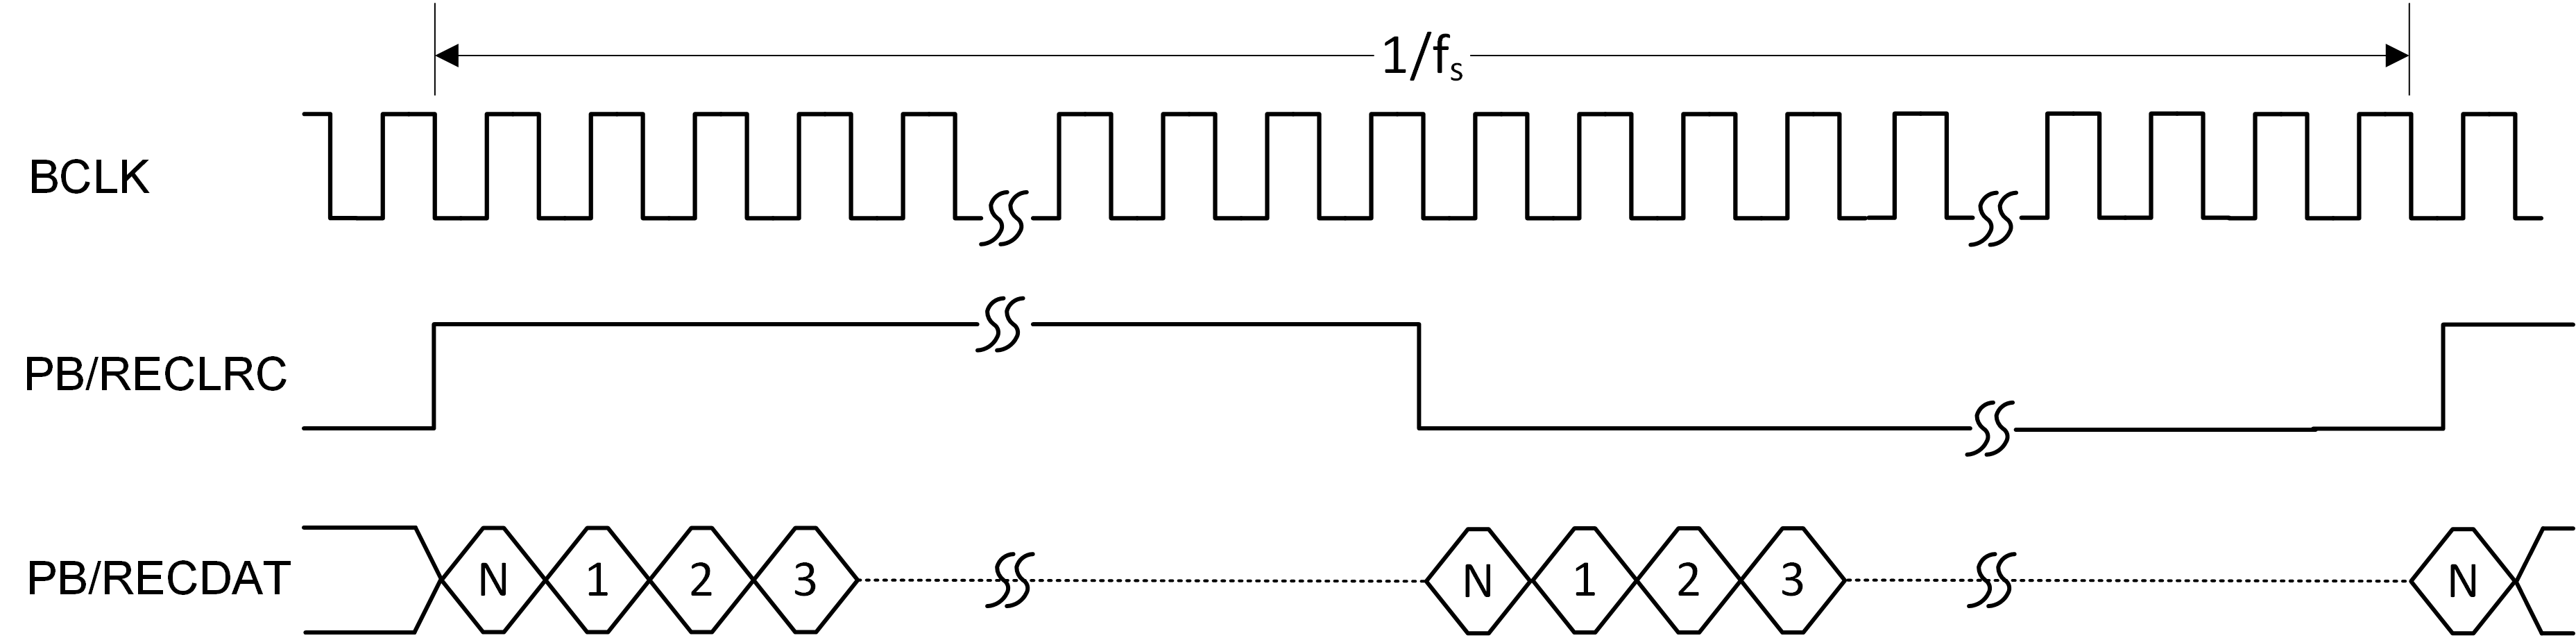
\includegraphics[width=.8\textwidth]{chapter06_figures/zybo-z7-audio.png}
  \end{center}
  \label{fig:ssm2603_protocol}
  \caption{SSM2603との通信インターフェース}
 \end{figure}
これを送受信するモジュールを実装して音声信号の入出力をやってみましょう.
でてくる信号が少し増えて複雑にみえるかもしれませんが,方針はRS-232-Cの送受信と同じです.

\subsection{I2Sの送信}
次のリストは,I2Sの送信モジュールの実装例です.シミュレーションによって,信号が図\ref{fig:ssm2603_protocol}に示したように出力されることを確認してみましょう.

\begin{figure}[H]
\begin{quote}
\begin{Verbatim}[frame=single, numbers=left, baselinestretch=0.8]
library ieee;

use ieee.std_logic_1164.all;
use ieee.numeric_std.all;

entity i2s_encoder is
  generic (
    WIDTH : integer := 24
    );
  port (
    CLK : in std_logic; -- BCLK 4x

    BCLK : in  std_logic;
    LRC  : in  std_logic;
    DAT  : out std_logic;

    LIN : in std_logic_vector(WIDTH-1 downto 0);
    RIN : in std_logic_vector(WIDTH-1 downto 0)
    );
end entity i2s_encoder;

architecture RTL of i2s_encoder is

  attribute mark_debug : string;

  signal left_data  : std_logic_vector(WIDTH-1 downto 0) := (others => '0');
  signal left_cnt   : unsigned(7 downto 0) := (others => '0');

  signal right_data  : std_logic_vector(WIDTH-1 downto 0) := (others => '0');
  signal right_cnt   : unsigned(7 downto 0) := (others => '0');
  
  signal lrc_d : std_logic := '0';
  signal bclk_d : std_logic := '0';

  attribute mark_debug of left_data  : signal is "true";
  attribute mark_debug of left_cnt   : signal is "true";
  
  attribute mark_debug of right_data  : signal is "true";
  attribute mark_debug of right_cnt   : signal is "true";

begin

  process(CLK)
  begin
    if rising_edge(CLK) then
\end{Verbatim}
\end{quote}
\end{figure}
次のページに続く
\begin{figure}[H]
\begin{quote}
\begin{Verbatim}[frame=single, numbers=left, baselinestretch=0.8]
      
      lrc_d  <= LRC;
      bclk_d <= BCLK;
      
      if lrc_d = '1' and LRC = '0' then
        left_cnt  <= (others => '0');
        left_data <= LIN;
      else
        if left_cnt <= 4*WIDTH-1 then
          left_cnt  <= left_cnt + 1;
          if 3 <= left_cnt then
            DAT        <= left_data(WIDTH-1);
            if left_cnt(1 downto 0) = "10" then
              left_data <= left_data(WIDTH-2 downto 0) & '0';
            end if;
          end if;
        end if;
      end if;
      
      if lrc_d = '0' and LRC = '1' then
        right_cnt  <= (others => '0');
        right_data <= RIN;
      else
        if right_cnt <= 4*WIDTH-1 then
          right_cnt  <= right_cnt + 1;
          if 3 <= right_cnt then
            DAT        <= right_data(WIDTH-1);
            if right_cnt(1 downto 0) = "10" then
              right_data <= right_data(WIDTH-2 downto 0) & '0';
            end if;
          end if;
        end if;
      end if;
      
    end if;
  end process;

end RTL;
\end{Verbatim}
\end{quote}
\end{figure}

\subsection{I2Sの受信}
次は受信モジュールです.送信モジュールと組み合わせてシミュレーションすることで,入力した音声信号をI2Sフォーマットに変換し,それが復号される様を観測することができます.

\begin{figure}[H]
\begin{quote}
\begin{Verbatim}[frame=single, numbers=left, baselinestretch=0.8]
library ieee;

use ieee.std_logic_1164.all;
use ieee.numeric_std.all;

entity i2s_decoder is
  generic (
    WIDTH : integer := 24
    );
  port (
    CLK : in std_logic;
    
    BCLK : in std_logic;
    LRC  : in std_logic;
    DAT  : in std_logic;

    LOUT : out std_logic_vector(WIDTH-1 downto 0);
    ROUT : out std_logic_vector(WIDTH-1 downto 0);
    LOUT_VALID : out std_logic;
    ROUT_VALID : out std_logic
    );
end entity i2s_decoder;

architecture RTL of i2s_decoder is

  attribute mark_debug : string;

  signal left_data  : std_logic_vector(WIDTH-1 downto 0) := (others => '0');
  signal left_cnt   : unsigned(5 downto 0) := (others => '0');
  signal left_valid : std_logic := '0';

  signal right_data  : std_logic_vector(WIDTH-1 downto 0) := (others => '0');
  signal right_cnt   : unsigned(5 downto 0) := (others => '0');
  signal right_valid : std_logic := '0';
  
  signal lrc_d : std_logic := '0';

  attribute mark_debug of left_data  : signal is "true";
  attribute mark_debug of left_valid : signal is "true";
  attribute mark_debug of left_cnt   : signal is "true";
  
  attribute mark_debug of right_data  : signal is "true";
  attribute mark_debug of right_valid : signal is "true";
  attribute mark_debug of right_cnt   : signal is "true";

\end{Verbatim}
\end{quote}
\end{figure}
次のページに続く
\begin{figure}[H]
\begin{quote}
\begin{Verbatim}[frame=single, numbers=left, baselinestretch=0.8]
  signal bclk_d : std_logic := '0';

begin

  LOUT_VALID <= left_valid;
  ROUT_VALID <= right_valid;
  
  LOUT <= left_data;
  ROUT <= right_data;

  process(CLK)
  begin
    if rising_edge(CLK) then
      bclk_d <= BCLK;

      if bclk_d = '0' and BCLK = '1' then
        
        left_data  <= left_data(WIDTH-2 downto 0) & DAT;
        right_data <= right_data(WIDTH-2 downto 0) & DAT;

        lrc_d <= LRC;
        
        if lrc_d = '1' and LRC = '0' then
          left_cnt <= (others => '0');
        else
          if left_cnt = WIDTH-1 then
            left_valid <= '1';
          else
            left_valid <= '0';
          end if;
          if left_cnt <= WIDTH-1 then
            left_cnt <= left_cnt + 1;
          end if;
        end if;
        
        if lrc_d = '0' and LRC = '1' then
          right_cnt <= (others => '0');
        else
          if right_cnt = WIDTH-1 then
            right_valid <= '1';
          else
            right_valid <= '0';
          end if;
          if right_cnt <= WIDTH-1 then
            right_cnt <= right_cnt + 1;
          end if;
        end if;
      end if;
    end if;
  end process;

end RTL;
\end{Verbatim}
\end{quote}
\end{figure}

\section{発展}
紹介したアプリケーション実験を応用して,次のような課題に挑戦してみましょう.

\begin{enumerate}
 \item ストップウォッチモジュールを改造して,カウントダウンできるようにしてみましょう.
 \item いろいろな通信速度でRS-232-C通信を試してみましょう.
 \item 音声入出力ができるようになったので,たとえば,規定値より大きな値がきたときだけ音声を出力する,平滑化フィルタで音を滑らかにする,などが簡単には考えられるでしょう.
\end{enumerate}


\end{document}
